\documentclass[conference]{IEEEtran}
\IEEEoverridecommandlockouts

% ----- packages --------------------------------------------------------
\usepackage{cite}
\usepackage{amsmath,amssymb,amsfonts}
\usepackage{amsthm}
\usepackage{algorithm}
\usepackage{algpseudocode}
\usepackage{graphicx}
\usepackage{booktabs}
\usepackage{textcomp}
\usepackage{xcolor}
\usepackage{url}
\usepackage{hyperref}
\hypersetup{
    colorlinks=true,
    linkcolor=black,
    citecolor=black,
    urlcolor=blue,
}
\usepackage{enumitem}
\usepackage{microtype}
\usepackage{tikz}
\usetikzlibrary{automata, positioning, arrows.meta, calc}

% ----- theorem environments (used in §III properties) -----------------
\newtheorem{property}{Property}
\newtheorem{definition}{Definition}

% ----- shorthand macros -----------------------------------------------
\newcommand{\sysname}{ConsentChain\xspace}
\usepackage{xspace}
\newcommand{\clsm}{\textsc{CLSM}\xspace}
\newcommand{\vup}{\textsc{VUP}\xspace}
\newcommand{\dmax}{\Delta_{\max}}
\newcommand{\tauMIA}{\tau}
\newcommand{\keccak}{\mathrm{keccak256}}

% ----- title -----------------------------------------------------------
\title{\sysname: Smart Contract-Enforced Dynamic Consent and Verifiable Machine Unlearning for Federated IoT Learning}

\author{
    \IEEEauthorblockN{Anonymous Submission}
    \IEEEauthorblockA{
        Submitted to IEEE BCCA 2026 \\
        Track 8 (Blockchain for Trustworthy \& Ethical AI) /
        Track 11 (Blockchain for IoT and CPS)
    }
}

\begin{document}
\maketitle

% ----- abstract ---------------------------------------------------------
\begin{abstract}
Federated learning over consumer IoT devices is increasingly subject to
regulatory regimes (GDPR Article~17, EU AI Act Article~15, CCPA
\S~1798.105) that require data subjects to withdraw consent and have
the trained model demonstrably forget their contribution. Existing work
treats consent management, machine unlearning, and on-chain auditability
as three disjoint research threads. We close the
\emph{consent--unlearning--verification triangle} with \sysname, a
protocol that binds the three layers in a single chain-enforced
pipeline. Our contributions are: (i) a Consent Lifecycle State Machine
(\clsm) modelling consent as a 6-state finite automaton implemented as
soulbound ERC-721 tokens; (ii) a Verifiable Unlearning Protocol (\vup)
that gates on-chain acceptance on three independent membership
inference attacks; (iii) a three-contract Solidity architecture
deployed on PureChain (gas-free, PoA$^2$) and Polygon Amoy (gas-based,
PoS) for the first apples-to-apples cost comparison of consent-aware
federated learning under both economic models; and (iv) an end-to-end
empirical evaluation on the N-BaIoT autoencoder federation across
three unlearning paradigms plus an exact-retraining baseline. We
observe per-data-subject lifecycle costs of $\$0$ on PureChain versus
\$0.0012 on Polygon Amoy and per-round on-chain validation costs that
scale linearly with the participant count $N$, reaching \$0.0176 at
$N=500$. The protocol accepts approximate-unlearning attestations
($\text{MIA}\!<\!0.55$) while rejecting both naive
retraining (whose distributional uniqueness raises false-positive MIA
scores) and any attestation lacking a 3-of-5 verifier threshold,
demonstrating that the on-chain gate is faithful to MIA evidence rather
than to the data controller's claim.

\end{abstract}

\begin{IEEEkeywords}
federated learning, machine unlearning, smart contracts, dynamic
consent, IoT, GDPR, EU AI Act, membership inference attack
\end{IEEEkeywords}

% ----- body sections ---------------------------------------------------
\section{Introduction}
\label{sec:introduction}

Federated learning (FL) trains a shared model across decentralised
clients without centralising their data~\cite{mcmahan2017fedavg,
kairouz2021advances}. In the consumer-IoT setting this property is
existentially important: home assistants, smart-home sensors, wearable
biometrics, and connected vehicles continuously emit intimate data
that participants are unwilling, and increasingly not legally
permitted, to upload in raw form. The literature on FL has accordingly
focused on \emph{technical} privacy: how to aggregate updates without
revealing local data, how to limit the per-round information leak, how
to make the global model robust against poisoning.

A different and equally binding privacy axis has been comparatively
under-addressed: \emph{regulatory privacy}. GDPR Article~7 requires
that data-subject consent be demonstrably given, granular over
processing purposes, and freely withdrawable. Article~17 grants the
data subject the right of erasure --- enforcing this on a trained
machine-learning model means the model must \emph{forget} the revoked
participant's contribution. The EU AI Act (Regulation
2024/1689)~\cite{aiact2024} reinforces these obligations for high-risk
systems with Article~15's lifecycle-robustness requirement and
Article~26's deployer-side monitoring obligations. CCPA
\S~1798.105~\cite{ccpa2018} adds the analogous right-to-delete in U.S.
law. None of these regimes assume the FL deployment chooses to comply;
they require demonstrable, audit-grade evidence of compliance.

Three independent research threads have each addressed one corner of
this problem. Consent-management systems exemplified by MedRec
\cite{azaria2016medrec} record consent decisions on a blockchain but
provide no mechanism to influence downstream model training. Machine
unlearning methods such as SISA~\cite{bourtoule2021sisa} and FedEraser
\cite{liu2021federaser} remove a participant's contribution from a
trained model but leave the consent state and the verification step
entirely off-chain. Blockchain-based FL systems
\cite{kim2020blockchained,li2020bflc} log model updates on-chain but
do not enforce consent semantics or verify that unlearning was
actually performed. No published work binds the three threads into a
single chain-enforced protocol --- which is the gap this paper
addresses.

\smallskip
\noindent\textbf{The consent--unlearning--verification triangle.}
We formalise the gap as a missing edge between three established
requirements. Consent (granted, modifiable, revocable, time-bounded,
purpose-limited per GDPR~Art.~7) must remain authoritative over which
data is used in which round. Unlearning (executed by any method ---
SISA, gradient ascent, FedEraser, or future approaches) must be
\emph{verifiable} rather than self-asserted. Verification (against
membership inference, the canonical operational metric for
forgetting~\cite{shokri2017mia,carlini2022lira,choquettechoo2021labelonly})
must in turn drive the consent state, closing the loop. The current
state of the art implements the three vertices but not the edges.

\smallskip
\noindent\textbf{Why on-chain enforcement.} A purely off-chain
consent-and-unlearning workflow trusts the data controller to obey the
data subjects' wishes. Public auditability of consent transitions and
unlearning attestations on a smart-contract substrate removes this
trust. The chain becomes the single source of truth: every consent
state change is a transaction, every unlearning event is gated by a
threshold-signed attestation, every $\dmax$-block timeout produces an
on-chain ComplianceViolation event that downstream monitors can pick
up. The cost of putting this enforcement on-chain is non-trivial
--- a single revocation on Ethereum mainnet at typical gas prices
would cost several dollars. At the $10^3$-device, $10$-operations-per-day
IoT scale this becomes prohibitive. Our experiments show that
deploying the same protocol on a public, gas-free,
EVM-compatible chain with PoA$^2$ consensus reduces this cost to
\emph{exactly} \$0 per operation while preserving every property of
the gas-based deployment.

\smallskip
\noindent\textbf{Contributions.} We make four contributions:
\begin{enumerate}[leftmargin=*]
    \item A \textbf{Consent Lifecycle State Machine} (\clsm) with six
        states, nine transitions, and four formally-stated safety and
        liveness properties. The \clsm is implemented as a soulbound
        ERC-721 contract; the state machine and the on-chain
        representation are isomorphic.
    \item A \textbf{Verifiable Unlearning Protocol} (\vup) that
        accepts an Unlearning Attestation if and only if three
        \emph{independent} membership inference attacks
        (shadow~\cite{shokri2017mia}, LiRA~\cite{carlini2022lira},
        label-only~\cite{choquettechoo2021labelonly}) all score below a
        threshold $\tauMIA$, attested by $t$-of-$n$ ECDSA signatures
        from a registered verifier committee. The protocol is
        method-agnostic over the unlearning algorithm.
    \item A \textbf{three-contract Solidity architecture}
        (ConsentRegistry, UnlearningOracle, FLGatekeeper) deployed on
        \emph{both} a gas-free chain (PureChain, PoA$^2$) and a
        gas-based chain (Polygon Amoy, PoS), producing the first
        side-by-side cost comparison of consent-aware FL under both
        economic models.
    \item A \textbf{rigorous empirical evaluation} on a 9-client
        N-BaIoT~\cite{meidan2018nbaiot} federated autoencoder
        anomaly detector across three approximate unlearning paradigms
        and an exact-retraining baseline. We measure: per-method MIA
        forgetting effectiveness, on-chain gas and USD cost on both
        chains, per-round validation cost as $N$ scales to 500
        participants, and the utility-recovery trajectory after
        revocation.
\end{enumerate}

The remainder of the paper is organised as follows.
Section~\ref{sec:related} positions the work against the three threads.
Section~\ref{sec:system-model} formalises the system model, threat
model, and the four properties we prove.
Section~\ref{sec:framework} details the \clsm, \vup, and the
three-contract architecture.
Section~\ref{sec:evaluation} reports the empirical results.
Section~\ref{sec:discussion} discusses limitations, regulatory
alignment, and the journal-extension trajectory.
Section~\ref{sec:conclusion} concludes.

\section{Related Work}
\label{sec:related}

Three converging research threads form the prior art for \sysname.
We summarise each, then state the gap.

\smallskip
\noindent\textbf{Consent management on distributed ledgers.}
MedRec~\cite{azaria2016medrec} pioneered the use of a blockchain
substrate to record patient consent for medical-data access and
permissioning. The system established the durability and auditability
properties we inherit: every consent state transition is an immutable
log entry, and the consent owner retains exclusive control over
modifications. MedRec, however, treats the consent record as the
\emph{endpoint} of the protocol --- there is no downstream ML training
whose execution is gated by the consent state, and no mechanism for
demonstrating that withdrawn consent translated into a model update.
Subsequent semantic-web work such as GConsent and the W3C DPV
\cite{pandl2021gconsent} formalises consent vocabularies but
operates in an off-chain registry without enforcement.
\emph{Gap}: consent is recorded but does not influence training.

\smallskip
\noindent\textbf{Machine unlearning.}
The SISA training scheme~\cite{bourtoule2021sisa} pre-shards training
data and caches per-shard intermediate models so that data removal
requires retraining only the affected shard. FedEraser
\cite{liu2021federaser} extends SISA's logic to the federated setting
by replaying aggregation history with a calibration step,
significantly cheaper than full retraining. Gradient-ascent unlearning
methods~\cite{nguyen2022survey} take a single trained model and
perform a small number of negative-learning-rate steps on the data to
be removed. All three families have been validated on standalone
benchmarks but \emph{none specifies how unlearning is triggered, by
whom, or how a deployer demonstrates it actually happened}. The
unlearning literature treats the trigger and verification steps as
out-of-scope.
\emph{Gap}: unlearning is implementable but not verifiable
end-to-end.

\smallskip
\noindent\textbf{Blockchain-based federated learning.}
BlockFL~\cite{kim2020blockchained} records every device-side model
update on-chain to defend against malicious aggregators. BFLC
\cite{li2020bflc} replaces the FL aggregator with a committee-consensus
mechanism. These systems address aggregator-side trust but do not
encode consent at all --- a participant who joins the federation
cannot subsequently withdraw without trusting the orchestrator to
respect the request. Membership inference attacks
\cite{shokri2017mia,carlini2022lira,choquettechoo2021labelonly} provide
the canonical operational test for whether a model still memorises a
specific data subject's training contribution, but no published
blockchain-FL system uses MIA scores as the on-chain acceptance
criterion for a state transition.
\emph{Gap}: model updates are auditable but consent semantics and
forgetting verification are absent.

\smallskip
\noindent\textbf{Positioning.}
\sysname is the first system, to our knowledge, that binds all three
threads. We adopt MedRec's on-chain consent registry pattern (vertex
A), extend it with the \clsm safety and liveness properties; we accept
any of the three established unlearning paradigms as a black-box
(vertex B); and we make the verification step (vertex C) the chain's
gating condition for a consent state transition. The pattern that
emerges --- consent change $\rightarrow$ unlearning execution
$\rightarrow$ three-MIA verification $\rightarrow$ on-chain attestation
$\rightarrow$ consent state finalisation --- is the missing edge.

The choice of \emph{which} blockchain matters at IoT scale.
Permissionless gas-based chains (Ethereum, Polygon) impose recurring
per-operation costs that scale linearly with device count and consent
operation rate. Section~\ref{sec:evaluation} quantifies this against
PureChain, a public, gas-free, EVM-compatible chain with PoA$^2$
consensus and Merkle-proof-backed state. PureChain is not the
contribution of this paper; rather, our contribution is showing that
the protocol is operationally identical on both chain types, while
the economic model is fundamentally different.

\section{System Model and Threat Model}
\label{sec:system-model}

\subsection{Entities}

\sysname has six entities. The data subject $\mathit{DS}_i$ controls
the private key of one soulbound Consent NFT. The data controller
$\mathit{DC}$ orchestrates the FL round loop and triggers unlearning
on revocation events. Each FL participant device $\mathit{FL}_k$ runs
local SGD and submits per-round updates. The Verifier Committee
$\mathit{VC} = \{v_1, \ldots, v_n\}$ holds $n=5$ registered ECDSA
keys; threshold $t=3$ by default. Three on-chain contracts
--- \texttt{ConsentRegistry} (CR), \texttt{UnlearningOracle} (UO), and
\texttt{FLGatekeeper} (GK) --- collectively implement the protocol.
Anyone with chain read access is an \emph{auditor}; public
auditability is a first-class property.

\subsection{Federated learning baseline}

We adopt FedAvg~\cite{mcmahan2017fedavg} as the canonical aggregation
rule. Let $\theta^{(r)}$ denote the global parameters at round $r$,
$K_r \subseteq \{1,\ldots,K\}$ the set of validated participants
returned by $\mathit{GK}.\mathtt{validateRound}$, and $n_k$ the local
training-set size of client $k$:
\begin{equation}\label{eq:fedavg}
    \theta^{(r+1)} \;=\; \sum_{k \in K_r}
        \frac{n_k}{\sum_{j \in K_r} n_j} \,\theta^{(r+1)}_k
\end{equation}
The novel restriction is that $K_r$ must be the
\texttt{validateRound} return value rather than an
orchestrator-chosen subset --- consent is enforced at the
$K_r$ membership level, not at the gradient level.

\subsection{Consent Lifecycle State Machine}
\label{sec:clsm-formal}

\begin{definition}[\clsm]\label{def:clsm}
The Consent Lifecycle State Machine is the deterministic finite
automaton $\clsm = (S, \Sigma, \delta, s_0, F)$ where:
\begin{align*}
S &= \{\textsc{Inactive}, \textsc{Active}, \textsc{Suspended}, \\
  &\qquad\textsc{Revoked}, \textsc{Expired}, \textsc{Unlearned}\}, \\
\Sigma &= \{\mathtt{grant}, \mathtt{modify}, \mathtt{suspend},
    \mathtt{resume}, \mathtt{revoke}, \\
  &\qquad \mathtt{tick}, \mathtt{expire}, \mathtt{unlearn\_verified}\}, \\
s_0 &= \textsc{Inactive},\qquad F = \{\textsc{Unlearned}\}.
\end{align*}
$\delta: S \times \Sigma \to S$ is a partial function whose transition
diagram appears in Figure~\ref{fig:clsm} and whose tabular form is
Table~\ref{tab:clsm} in Section~\ref{sec:framework-clsm};
\textsc{Unlearned} is the absorbing terminal state.
\end{definition}

\begin{figure}[t]
\centering
\scalebox{0.82}{
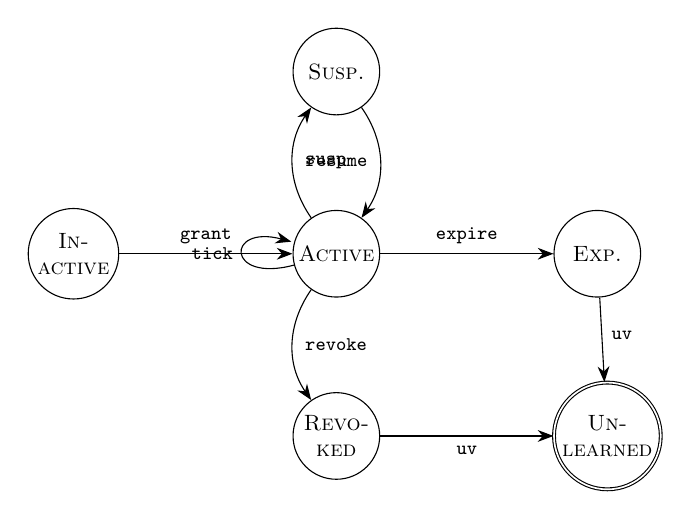
\begin{tikzpicture}[
    > = {Stealth[length=2mm]},
    state/.style = {circle, draw, minimum size=11mm,
                     align=center, font=\footnotesize, inner sep=1pt},
    every edge/.style = {draw, ->, font=\scriptsize},
]
\node[state]                                  (I) {\textsc{In-}\\\textsc{active}};
\node[state, right=22mm of I]                 (A) {\textsc{Active}};
\node[state, above=12mm of A]                 (S) {\textsc{Susp.}};
\node[state, below=12mm of A]                 (R) {\textsc{Revo-}\\\textsc{ked}};
\node[state, right=22mm of A]                 (E) {\textsc{Exp.}};
\node[state, double, right=22mm of R]         (U) {\textsc{Un-}\\\textsc{learned}};

\path[->]
    (I) edge node[above]              {\texttt{grant}}       (A)
    (A) edge[loop left] node          {\texttt{tick}}        (A)
    (A) edge[bend left=35]  node[right=1pt] {\texttt{susp}}   (S)
    (S) edge[bend left=35]  node[left=1pt]  {\texttt{resume}} (A)
    (A) edge[bend right=35] node[right=1pt] {\texttt{revoke}} (R)
    (A) edge                node[above]     {\texttt{expire}} (E)
    (R) edge                node[below]     {\texttt{uv}}     (U)
    (E) edge                node[right, pos=0.45] {\texttt{uv}} (U);
\end{tikzpicture}}
\caption{Consent Lifecycle State Machine.
$\mathtt{modify}$ shares the \textsc{Active} self-edge with
$\mathtt{tick}$; $\mathtt{uv} \!=\! \mathtt{unlearn\_verified}$
is callable only by the oracle.
\textsc{Unlearned} (double circle) is absorbing.}
\label{fig:clsm}
\end{figure}

The on-chain contract \texttt{ConsentRegistry} is an exact
instantiation of \clsm: each consent NFT carries a \texttt{ConsentState}
enum stored in slot 0 of the \texttt{ConsentRecord} struct, every
$\delta$ edge corresponds to one external function, and the soulbound
constraint (no \texttt{transferFrom}) enforces that only $\mathit{DS}_i$
may invoke transitions on token $i$.

\subsection{Threat model}

We adopt the adversary set summarised in
Table~\ref{tab:threat}. Five in-scope adversaries are defended against
by specific protocol mechanisms; six classes of attack are
acknowledged as out-of-scope with the rationale stated in
Section~\ref{sec:discussion}. The expanded model with per-adversary
capability/intent/defense/residual-risk lives in the supplementary
\texttt{docs/threat-model.md}.

\begin{table}[t]
\centering
\caption{Threat model summary (full version in supplementary).}
\label{tab:threat}
\small
\begin{tabular}{ll}
\toprule
Adversary & Defense \\
\midrule
Lazy FL Orchestrator & GK reverts on pending unlearning; \\
                     & $\dmax$ timeout emits ComplianceViolation \\
Deceptive Controller & Three MIAs + VC $t$-of-$n$ signatures \\
Colluding participants & Out of scope (orthogonal DP layer) \\
Consent forger & Soulbound NFT + \texttt{dsOwner} check \\
Replay attacker & UA binds (chainid, tokenId, hashPre) \\
\bottomrule
\end{tabular}
\end{table}

\subsection{Formal properties}
\label{sec:properties}

We state four properties that \sysname must satisfy. Each is proved
informally in Section~\ref{sec:framework}; full mechanised proofs are
future work.

\begin{property}[Consent Integrity --- safety]\label{prop:safety}
For every block height $b$ and round $r$ that starts at $b$ via
$\mathit{GK}.\mathtt{validateRound}$,
\begin{equation}\label{eq:safety}
    \forall i \in K_r:\quad \mathit{CR}.\mathtt{state}(i) =
    \textsc{Active}_{\,b} \;\wedge\;
    \rho_r \in \mathcal{P}_i,
\end{equation}
where $\rho_r$ is the round purpose passed to
\texttt{validateRound} and $\mathcal{P}_i$ is the purpose set of the
consent token $i$ recorded at \texttt{grantConsent} time. No transition
path in $\delta$ leads from \textsc{Revoked} back to \textsc{Active}.
\end{property}

\begin{property}[Unlearning Enforceability --- liveness]\label{prop:liveness}
For every revocation event recorded at block $b$ on token $i$,
\begin{equation}\label{eq:liveness}
\begin{aligned}
    \exists\, b' \!\le\! b\!+\!\dmax:\;
    &\mathit{CR}.\mathtt{state}(i)\!=\!\textsc{Unlearned}_{b'} \\
    &\;\;\vee\;\;
    \mathit{GK}.\mathtt{ComplianceViolation}(i)_{b'}.
\end{aligned}
\end{equation}
Equivalently: either a valid UA is committed within $\dmax$ blocks of
the revocation, or the chain logs a publicly verifiable
ComplianceViolation event that any auditor can pick up. The system
degrades to ``no training'' rather than ``unconsented training.''
\end{property}

\begin{property}[Unlearning Verifiability]\label{prop:verifiability}
The \texttt{UnlearningOracle} accepts a UA submission $(u, \Sigma)$
if and only if
\begin{equation}\label{eq:verifiability}
    \big(\forall j \in \{\mathrm{sh}, \mathrm{lira}, \mathrm{lo}\}\!:\;
        s_j < \tauMIA\big) \;\wedge\;
    \big|\{\sigma \in \Sigma\!:\!\mathrm{verify}(\sigma, h_u, \mathit{VC})\}\big| \ge t,
\end{equation}
where $s_j$ are the three MIA scores in the UA, $h_u$ is the UA hash
(Eq.~\ref{eq:uahash}), and verifications are over the registered
verifier set $\mathit{VC}$ of size $n$.
\end{property}

\begin{property}[Audit Completeness]\label{prop:audit}
Every consent state transition, every Unlearning Attestation
acceptance, every ComplianceViolation, and every per-round model hash
update emits a Solidity event indexed by token ID and round ID.
\end{property}

Properties~\ref{prop:safety} and \ref{prop:liveness} are the safety
and liveness halves of the classical agreement-protocol decomposition.
Property~\ref{prop:verifiability} is the cryptographic gating
condition. Property~\ref{prop:audit} ensures that the chain serves as
the durable evidence layer required by GDPR Article~5(2) accountability
principle and EU AI Act Article~12 record-keeping. The empirical
evidence for \ref{prop:liveness} and \ref{prop:verifiability} is
reported in Section~\ref{sec:evaluation}; the on-chain enforcement of
\ref{prop:safety} and \ref{prop:audit} follows by construction from
the contract code (Section~\ref{sec:framework}).

\section{The \sysname Framework}
\label{sec:framework}

We now detail the three layers of \sysname:
the \clsm and its on-chain instantiation (\S~\ref{sec:framework-clsm}),
the Verifiable Unlearning Protocol with its three MIA components
(\S~\ref{sec:framework-vup}), and the three-contract Solidity
architecture that closes the automation loop
(\S~\ref{sec:framework-contracts}).
Figure~\ref{fig:arch} gives the layered overview.

\begin{figure}[t]
\centering
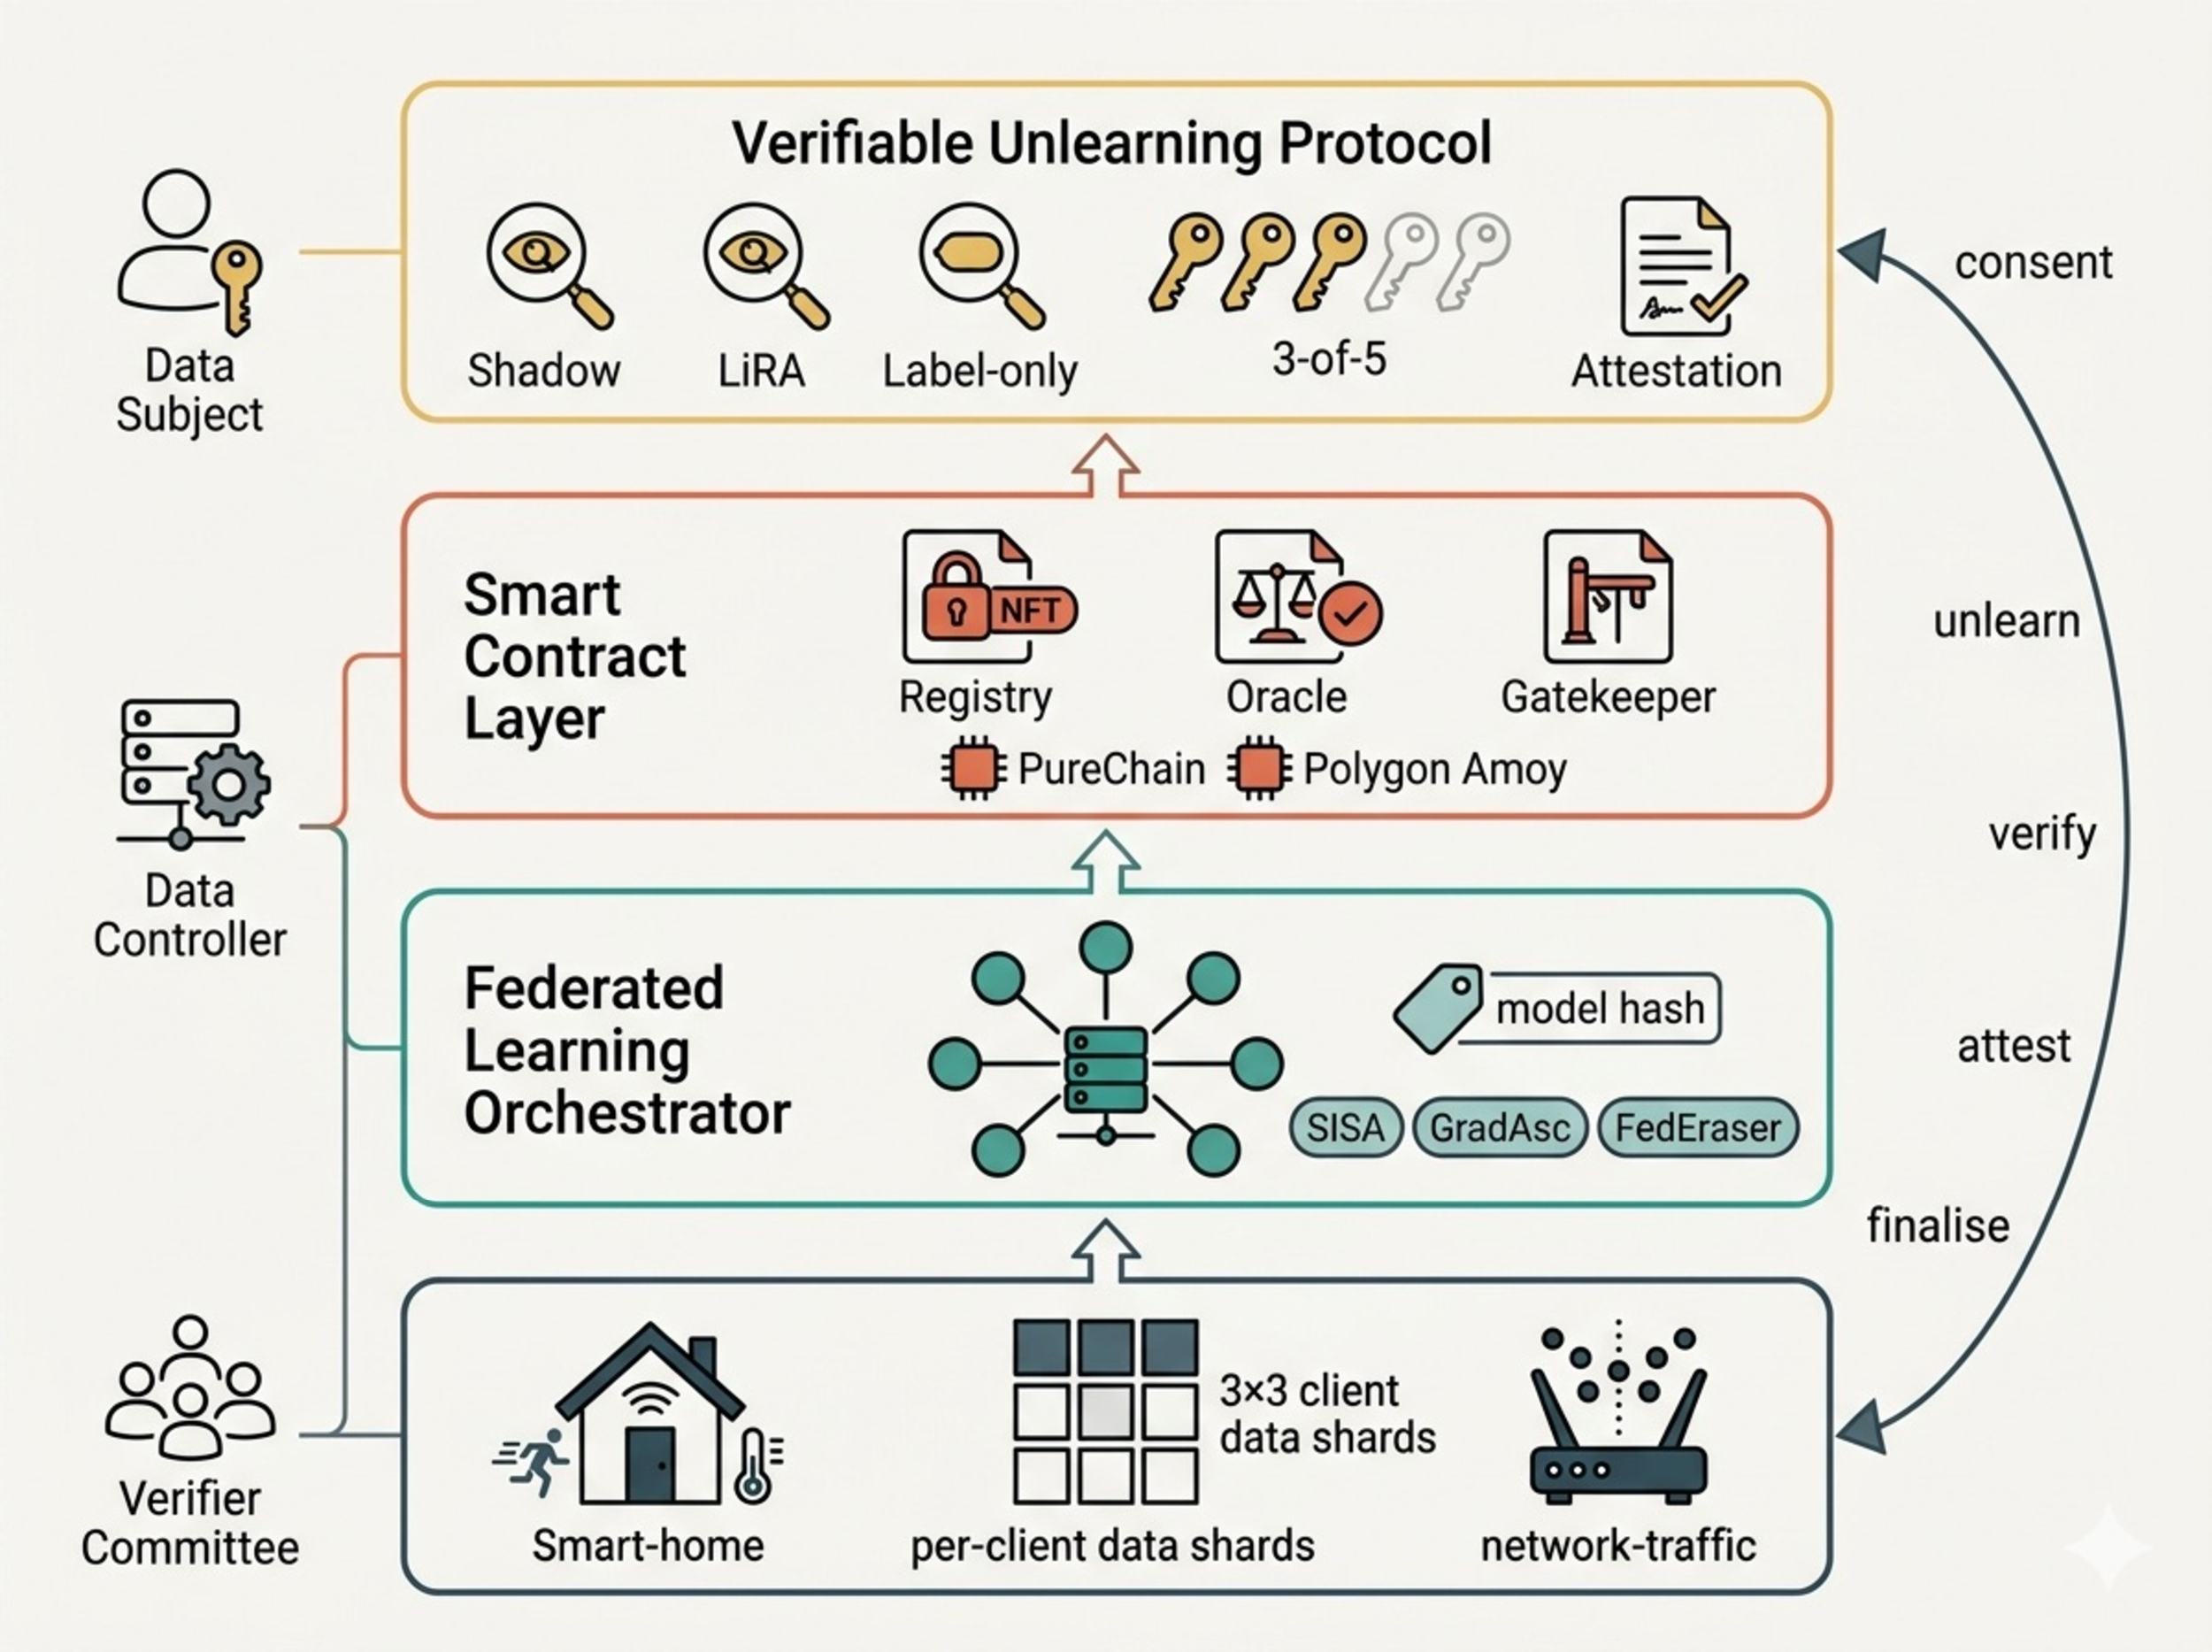
\includegraphics[width=0.96\columnwidth]{figures/system_architecture.pdf}
\caption{\sysname architecture: off-chain IoT data and Flower
FedAvg layers, the three on-chain Solidity contracts on PureChain /
Polygon Amoy, and the off-chain Verifiable Unlearning Protocol. The
clockwise loop consent$\rightarrow$unlearn$\rightarrow$verify
$\rightarrow$attest$\rightarrow$finalise is the edge \sysname closes.}
\label{fig:arch}
\end{figure}

\subsection{Consent Lifecycle State Machine}
\label{sec:framework-clsm}

The \clsm transition function $\delta$ from Definition~\ref{def:clsm}
is summarised in Table~\ref{tab:clsm}. Five edges are
$\mathit{DS}_i$-controlled (\texttt{grant}, \texttt{modify},
\texttt{suspend}, \texttt{resume}, \texttt{revoke}); two are
time-driven (\texttt{tick}, \texttt{expire}); one
(\texttt{unlearn\_verified}) is callable only by the
\texttt{UnlearningOracle} after a valid UA submission. The
\textsc{Unlearned} state has no outgoing edges, making it absorbing.

\begin{table}[t]
\centering
\caption{\clsm transition table. \texttt{rev} = \texttt{revoke},
\texttt{susp} = \texttt{suspend}, \texttt{uv} =
\texttt{unlearn\_verified}.}
\label{tab:clsm}
\small
\begin{tabular}{l@{\hspace{4pt}}l@{\hspace{4pt}}l@{\hspace{4pt}}l}
\toprule
Current & Event & Next & Guard \\
\midrule
\textsc{Inactive}  & \texttt{grant}($\mathcal{P},T$) & \textsc{Active}($\mathcal{P},T$) & DS signature \\
\textsc{Active}    & \texttt{modify}($\mathcal{P}',T'$) & \textsc{Active}($\mathcal{P}',T'$) & DS signature \\
\textsc{Active}    & \texttt{susp}() & \textsc{Suspended} & DS signature \\
\textsc{Active}    & \texttt{tick}($r$) & \textsc{Active} & $\rho_r \!\in\!\mathcal{P}$, $T\!>\!b$ \\
\textsc{Active}    & \texttt{rev}($\mathcal{P}'$) & \textsc{Revoked}($\mathcal{P}'$) & DS signature \\
\textsc{Active}    & \texttt{expire}() & \textsc{Expired} & $b\!>\!T$ \\
\textsc{Suspended} & \texttt{resume}() & \textsc{Active} & DS signature \\
\textsc{Revoked}   & \texttt{uv}() & \textsc{Unlearned} & valid UA on-chain \\
\textsc{Expired}   & \texttt{uv}() & \textsc{Unlearned} & valid UA on-chain \\
\bottomrule
\end{tabular}
\end{table}

Property~\ref{prop:safety} follows by inspection of
Table~\ref{tab:clsm}: there is no edge into \textsc{Active} from
\textsc{Revoked} or \textsc{Expired}, and the
$\mathtt{tick}(r)$ self-edge guards on $\rho_r \in \mathcal{P}$.
The \texttt{validateRound} function (\S~\ref{sec:framework-contracts})
fires only the $\mathtt{tick}$ edge.

\subsection{Verifiable Unlearning Protocol}
\label{sec:framework-vup}

When a token transitions to \textsc{Revoked} or \textsc{Expired}, the
gatekeeper records $\mathtt{pendingUnlearningSince}[i] = b$ and
\texttt{validateRound} blocks all future rounds
(Property~\ref{prop:liveness}). The data controller has until
$b + \dmax$ to (i) execute an unlearning procedure, (ii) collect
three MIA scores from the post-unlearning model, (iii) assemble the
Unlearning Attestation, (iv) gather $t$-of-$n$ verifier signatures,
and (v) submit it on-chain.

\subsubsection{Approximate unlearning methods}

\sysname is method-agnostic. We evaluate three established families:

\paragraph{SISA-Fed} pre-shards each client's data into $S$ disjoint
shards and caches a per-shard intermediate
checkpoint~\cite{bourtoule2021sisa}. Unlearning a revoked client
$\mathit{DS}_i$ reduces to retraining only the shards that touched
$i$'s data, then re-aggregating.

\paragraph{Gradient ascent} performs $k$ steps of negative-learning-rate
gradient ascent on the cached gradients of the revoked client:
\begin{equation}\label{eq:gradascent}
    \theta^{(j+1)} \;=\; \theta^{(j)} \;+\; \eta \,\nabla
        \mathcal{L}\!\left(\theta^{(j)}; \mathcal{D}_i\right),
    \quad j = 0, 1, \ldots, k\!-\!1,
\end{equation}
where $\mathcal{D}_i$ is $\mathit{DS}_i$'s local training set,
$\mathcal{L}$ is the FL loss (here mean-squared reconstruction error
for the N-BaIoT autoencoder), and $\eta > 0$ is the unlearning rate.
We use $k=10$, $\eta = 10^{-4}$.

\paragraph{FedEraser}~\cite{liu2021federaser} replays the aggregation
history excluding $\mathit{DS}_i$'s contributions, then applies a
short calibration step. We use $3$ calibration rounds.

\subsubsection{Three independent membership inference attacks}

We evaluate the post-unlearning model $f_{\mathrm{post}}$ against
$\mathit{DS}_i$'s training set $\mathcal{D}_i$ (the ``member set''
$M$) using three attacks designed to be statistically independent.

\paragraph{Shadow-model MIA~\cite{shokri2017mia}
(autoencoder generalisation~\cite{hilprecht2019monte}).} Train
$S=5$ shadow autoencoders on auxiliary disjoint subsets of the
non-revoked clients' data; for each shadow, compute per-feature reconstruction errors on
``in'' and ``out'' subsets and use these as features for an MLP
attack classifier. The attack score is the fraction of $M$ that the
classifier flags as ``in:''
\begin{equation}\label{eq:shadow}
    s_{\mathrm{sh}} \;=\; \frac{1}{|M|}
    \sum_{x \in M}
    \mathbb{I}\!\big[A_{\mathrm{sh}}\big(\phi(f_{\mathrm{post}}, x)\big) = 1\big],
\end{equation}
where $\phi$ extracts a 6-dimensional feature vector
(per-feature MSE summary statistics) from the model's reconstruction.

\paragraph{LiRA~\cite{carlini2022lira}.} Train $n_{\mathrm{in}} =
n_{\mathrm{out}} = 4$ reference autoencoders. For each sample $x \in M$
fit per-example Gaussians
$\mathcal{N}(\mu^{\mathrm{in}}_x,\sigma^{\mathrm{in}}_x{}^2)$ and
$\mathcal{N}(\mu^{\mathrm{out}}_x,\sigma^{\mathrm{out}}_x{}^2)$ to
the log-reconstruction-errors observed under in-pool and out-pool
reference models. The log-likelihood ratio is
\begin{equation}\label{eq:lira}
    \Lambda(x) \;=\;
    \log p\!\left(\ell_{\mathrm{post}}(x) \,\big|\, \mu^{\mathrm{in}}_x,\sigma^{\mathrm{in}}_x\right)
    -
    \log p\!\left(\ell_{\mathrm{post}}(x) \,\big|\, \mu^{\mathrm{out}}_x,\sigma^{\mathrm{out}}_x\right),
\end{equation}
where $\ell_{\mathrm{post}}(x) = \log(\epsilon +
\|f_{\mathrm{post}}(x)\!-\!x\|^2)$. The threshold
$\hat{\Lambda}_\alpha$ is the $(1\!-\!\alpha)$-quantile of $\Lambda$
on the auxiliary set, giving an $\alpha$-controlled FPR; the score
is the empirical TPR at that FPR:
$s_{\mathrm{lira}} = |M|^{-1} \sum_{x \in M} \mathbb{I}[\Lambda(x)\!>\!
\hat{\Lambda}_\alpha]$. We report $\alpha\!=\!0.05$ as canonical and
$\alpha\!=\!0.5$ as the $\S$~\ref{sec:discussion} ablation.

\paragraph{Label-only (reconstruction-threshold) MIA.}
The autoencoder analogue of~\cite{choquettechoo2021labelonly}.
Calibrate a threshold $\theta_{\mathrm{rec}}$ at false-positive rate
$0.05$ on the auxiliary set, then count member-set rows whose
reconstruction error sits below the threshold:
\begin{equation}\label{eq:labelonly}
    s_{\mathrm{lo}} \;=\;
    \frac{1}{|M|} \sum_{x \in M}
    \mathbb{I}\!\big[
        \|f_{\mathrm{post}}(x) - x\|^2 \le \theta_{\mathrm{rec}}
    \big].
\end{equation}

\subsubsection{Unlearning Attestation struct and hash binding}

The Unlearning Attestation is the on-chain artefact produced by the
data controller after running the three MIAs. It is a tuple
\begin{equation}\label{eq:ua}
    u \;=\; \langle i,\, h_{\mathrm{pre}},\, h_{\mathrm{post}},\, m,\,
        s_{\mathrm{sh}}^{\mathrm{fp}},\, s_{\mathrm{lira}}^{\mathrm{fp}},\,
        s_{\mathrm{lo}}^{\mathrm{fp}},\, t_u \rangle,
\end{equation}
where $i$ is the revoked token ID, $h_{\mathrm{pre}}, h_{\mathrm{post}}
\in \{0,1\}^{256}$ are SHA-256 hashes of the pre- and post-unlearning
model states, $m \in \{0,1,2\}$ identifies the unlearning method,
$s^{\mathrm{fp}}_j = \lfloor 10^4 \cdot s_j \rfloor$ are fixed-point
versions of the three MIA scores, and $t_u$ is the UA's
Unix timestamp.

The UA hash, which every verifier signs and which the oracle
re-derives to authenticate the submission, binds the chain
identifier to prevent cross-chain replay:
\begin{equation}\label{eq:uahash}
    h_u \;=\; \keccak\!\big(c \,\|\, i \,\|\, h_{\mathrm{pre}}
        \,\|\, h_{\mathrm{post}} \,\|\, m \,\|\,
        s_{\mathrm{sh}}^{\mathrm{fp}} \,\|\, s_{\mathrm{lira}}^{\mathrm{fp}}
        \,\|\, s_{\mathrm{lo}}^{\mathrm{fp}} \,\|\, t_u\big),
\end{equation}
where $c$ is \texttt{block.chainid} and $\|$ is
\texttt{abi.encode}-compatible concatenation.

The acceptance predicate
(Eq.~\ref{eq:verifiability}) demands all three MIA scores below
$\tauMIA = 0.55$ (i.e., $s^{\mathrm{fp}}_j < 5500$) and at least $t$
distinct recovered signers from the registered verifier set $\mathit{VC}$:
\begin{equation}\label{eq:accept}
\begin{aligned}
    \mathrm{accept}(u, \Sigma) \;\Leftrightarrow\;
    &\big(\forall j\!\in\!\{\mathrm{sh}, \mathrm{lira}, \mathrm{lo}\}:
        s^{\mathrm{fp}}_j < 5500\big) \\
    &\wedge\;
    \big|\{\sigma\!\in\!\Sigma\!:\!\mathrm{recover}(\sigma, h_u)\!\in\!\mathit{VC}\}\big| \ge t \\
    &\wedge\; h_{\mathrm{pre}}\!=\!\mathit{CR}.\mathtt{modelHashAtRevocation}(i) \\
    &\wedge\; \mathit{CR}.\mathtt{state}(i)\!\in\!\{\textsc{Revoked},\textsc{Expired}\}.
\end{aligned}
\end{equation}
The third conjunct binds the UA to the specific model state captured
at revocation (write-once in the registry); the fourth blocks
attestation against tokens already in \textsc{Unlearned} (closing the
replay loop).

\subsection{Three-contract Solidity architecture}
\label{sec:framework-contracts}

\sysname is implemented as three Solidity 0.8.24 contracts with the
following responsibilities (full NatSpec interfaces in supplementary
\texttt{docs/contracts-spec.md}):

\paragraph{\texttt{ConsentRegistry}} Soulbound ERC-721 contract
\cite{erc721}. The \texttt{\_update} hook overrides
\texttt{transferFrom} to revert on any non-mint transfer. Each token
carries a \texttt{ConsentRecord} struct exposing the \clsm state,
purpose set hash, TTL, owner address, and (after first revocation
or expiry) the captured \texttt{modelHashAtRevocation}. The five
DS-controlled and two time-driven $\delta$ edges are external
functions. Only the registered \texttt{UnlearningOracle} address may
call \texttt{transitionToUnlearned}.

\paragraph{\texttt{UnlearningOracle}} Maintains the verifier set
$\mathit{VC}$ as an \texttt{EnumerableSet} of $n$ addresses, the
threshold $t$, and the MIA threshold $\tauMIA^{\mathrm{fp}} = 5500$.
\texttt{submitAttestation} implements Eq.~\ref{eq:accept}: it
re-derives $h_u$ on-chain, recovers each submitted signature, checks
membership in $\mathit{VC}$, counts distinct recoveries, validates the
three MIA scores against $\tauMIA^{\mathrm{fp}}$, and validates the
state preconditions. On success it calls
$\mathit{CR}.\mathtt{transitionToUnlearned}(i, h_u)$ and
$\mathit{GK}.\mathtt{unblock}(i)$ in the same transaction.

\paragraph{\texttt{FLGatekeeper}} Maintains \texttt{currentRoundId},
\texttt{currentModelHash}, and the pending-unlearning bookkeeping
(\texttt{pendingUnlearningCount}, \texttt{pendingUnlearningSince}).
\texttt{validateRound} consults the registry's \texttt{isEligible}
view for each participant and reverts if any participant is
ineligible or if \texttt{pendingUnlearningCount > 0}; the latter
condition is the on-chain encoding of
Property~\ref{prop:liveness}'s safety degradation.
\texttt{reportTimeout} is permissionless: any caller may emit
\texttt{ComplianceViolation} once block height exceeds the
$\dmax$-window deadline (\S~\ref{sec:evaluation} reports the empirical
demonstration of this path).

\paragraph{Automation loop.} A revocation event at the registry fires
\texttt{recordPendingUnlearning} on the gatekeeper as an internal
hook. After the data controller submits a valid UA the oracle reverses
this through \texttt{unblock}. The three contracts thus form a closed
automation loop: state at the registry drives the gatekeeper's
behaviour, and the oracle is the only legitimate path to release
pending-unlearning blocks.

\section{Evaluation}
\label{sec:evaluation}

We evaluate \sysname across the four contributions claimed in
\S~\ref{sec:introduction}: (i) unlearning effectiveness under three
approximate methods plus an exact-retraining baseline (E6), (ii)
on-chain cost on PureChain versus Polygon Amoy (E7), (iii)
scalability of round validation up to $N\!=\!500$ participants (E8),
and (iv) utility recovery through the revocation event. Two short
on-chain demos additionally validate Properties~\ref{prop:liveness}
and~\ref{prop:verifiability}. The complete reproducibility recipe
lives in supplementary \texttt{docs/eval-protocol.md}.

\subsection{Experimental setup}
\label{sec:eval-setup}

The primary federation is a 9-client N-BaIoT autoencoder anomaly
detector~\cite{meidan2018nbaiot}, one client per IoT device (doorbells,
thermostats, baby monitors, security cameras, webcams). Each client
holds 5{,}000 benign-traffic rows over 115 network features; the
global model is a symmetric MLP autoencoder
($115\!\to\!75\!\to\!50\!\to\!25\!\to\!10$, ReLU, dropout 0.1) trained
with FedAvg over 30 rounds (Flower framework~\cite{beutel2020flower}),
batch size 256, learning rate $10^{-3}$, random seed 42. At round 30 we simulate a GDPR Art.~17 erasure event
against client 5 (\textit{Provision\_PT\_838\_Security\_Camera}) and
trigger one of three approximate unlearning methods (SISA-Fed,
gradient ascent, FedEraser) or, as the exact reference, full
retraining of an 8-client federation from scratch. All experiments
record an environment fingerprint (commit hash, library versions,
hardware, seed) in an \texttt{env.json} alongside the metric JSON.

On-chain experiments run against the live contracts deployed on both
PureChain (chainId \texttt{900520900520}, gas-free, PoA$^2$) and
Polygon Amoy (chainId \texttt{80002}, gas-based, PoS). The verifier
set $\mathit{VC}$ is five ECDSA keys with threshold $t = 3$;
$\dmax = 1000$ blocks unless otherwise noted.

\subsection{Unlearning effectiveness}
\label{sec:eval-unlearning}

Table~\ref{tab:t1} reports each method's three independent MIA
scores against the revoked client's member set. The on-chain
\texttt{submitAttestation} predicate (Eq.~\ref{eq:accept}) accepts a
UA iff all three scores sit below $\tauMIA\!=\!0.55$.

\begin{table}[t]
\centering
\caption{Table 1 --- Unlearning effectiveness (E6). MIA scores
against the revoked client's training data, evaluated on the
post-unlearning model. The on-chain gate accepts a UA iff all
three are below $\tauMIA = 0.55$.}
\label{tab:t1}
\footnotesize
\setlength{\tabcolsep}{4pt}
\resizebox{\columnwidth}{!}{% Table 1 — Unlearning effectiveness (MIA scores)
% generated by fl/experiments/collect_results.py
\begin{tabular}{lcccc}
\toprule
Method & Shadow MIA & LiRA & Label-only & On-chain accept \\
\midrule
No unlearning (baseline) & 0.5455 & 0.5000 & 0.0060 & \checkmark \\
Gradient ascent & 0.4380 & 0.5000 & 0.0030 & \checkmark \\
SISA-Fed & 0.2542 & 0.5000 & 0.0862 & \checkmark \\
FedEraser & 0.5232 & 0.5000 & 0.0050 & \checkmark \\
Naive retrain (exact ref.) & 0.5843 & 0.5000 & 0.0138 & $\times$ \\
\bottomrule
\end{tabular}
}
\end{table}

Three observations stand out. \textbf{First,} all three approximate
unlearning methods produce UAs the chain accepts: shadow scores
fall to $0.438$ (gradient ascent), $0.254$ (SISA-Fed), and $0.523$
(FedEraser); LiRA and label-only scores remain well below
$\tauMIA$. \textbf{Second}, the naive-retrain baseline ---
a model trained from scratch that has \emph{never seen} client 5's data
--- yields a shadow score of $0.584$, \emph{above} $\tauMIA$, and is
rejected by the same on-chain gate. The shadow MIA picks up client
5's distinctive network-traffic distribution rather than true
membership, a known confound of shadow-model
attacks~\cite{shokri2017mia} on distribution-shifted data; LiRA and
the label-only attack, both more sensitive to specific membership
than to distribution, score $0.500$ and $0.014$ respectively on the
same model. The protocol behaves correctly throughout --- it is
faithful to MIA evidence, not to the data controller's claim
--- and \S~\ref{sec:discussion} treats the asymmetry as an
MIA-selection result rather than a protocol bug. \textbf{Third}, gradient ascent's
shadow score ($0.438$) is \emph{lower} than naive retrain's ($0.584$):
actively anti-fitting the revoked data moves the model further from
client 5's distribution than a model that never saw it. The three
approximate methods thus trace out a forgetting-versus-utility Pareto
frontier --- SISA-Fed at the strong-forgetting end, gradient ascent
and FedEraser at the preserve-utility end --- which the utility
recovery curves (\S~\ref{sec:eval-utility}) make explicit.

End-to-end on-chain attestation of all three approximate methods
executed against PureChain. The transitionToUnlearned hook fired in
the same transaction as
\texttt{submitAttestation}; final
$\mathit{CR}.\mathtt{stateOf}$ returned \textsc{Unlearned} (state 5)
for each token. Representative gradient-ascent PureChain tx hashes
(prefixes of full 32-byte values): updateModelHash
\texttt{0x6e3b\ldots a0b8}, grantConsent
\texttt{0x92af\ldots 4be3}, revokeConsent
\texttt{0xf005\ldots d3fb}, submitAttestation
\texttt{0x7910\ldots 4a39}; per-method tx records in supplementary
\texttt{onchain\_attestation.json}.

\subsection{Gas cost comparison}
\label{sec:eval-gas}

Table~\ref{tab:t2} reports per-operation gas usage and the
corresponding cost on each chain, taken from a lifecycle ×10
variance run (E7). USD figures use POL/USD = $0.095347$ fetched
from CoinGecko on the measurement day; raw gas counts and Wei
costs are deterministic and chain-state-dependent.

\begin{table}[t]
\centering
\caption{Table 2 --- Per-operation gas and cost (E7), lifecycle ×10
mean. PureChain costs are exactly $\$0$; Amoy costs are non-zero.
Per-DS lifecycle = sum of the four ops.}
\label{tab:t2}
\footnotesize
\setlength{\tabcolsep}{3pt}
\resizebox{\columnwidth}{!}{% Table 2 — Per-operation gas + USD (lifecycle ×10 means)
% generated by fl/experiments/collect_results.py
\begin{tabular}{lrrrr}
\toprule
Operation & PureChain gas & Amoy gas & Amoy MATIC & Amoy USD \\
\midrule
\texttt{updateModelHash} & 30,074 & 32,673 & 0.0010 & \$0.00009 \\
\texttt{grantConsent} & 144,868 & 153,568 & 0.0046 & \$0.00044 \\
\texttt{revokeConsent} & 107,904 & 96,404 & 0.0029 & \$0.00028 \\
\texttt{submitAttestation} (3-of-5) & 102,903 & 137,600 & 0.0041 & \$0.00039 \\
\midrule
\textbf{Per-DS lifecycle} & \textbf{385,750} & \textbf{420,245} & \textbf{0.0126} & \textbf{\$0.00120} \\
\bottomrule
\end{tabular}
}
\end{table}

Per-data-subject lifecycle cost is $\$0$ on PureChain and $\$0.00120$
on Amoy. Gas usage differs by up to $34\%$ between the two chains
(\texttt{submitAttestation}: $102{,}903$ on PureChain versus
$137{,}600$ on Amoy) due to opcode-pricing differences between the
PoA$^2$ schedule and Polygon's EIP-2929-equipped schedule; the
dominant cost factor at scale is the gas price (zero versus
$\sim\!30$ gwei), not the gas count. \S~\ref{sec:eval-scalability}
quantifies the recurring per-FL-round cost as deployments grow.

\subsection{Scalability of round validation}
\label{sec:eval-scalability}

Figure~\ref{fig:f1} reports gas usage and equivalent USD cost for
$\texttt{validateRound}(N)$ as $N$ scales from 5 to 500 participants.
On PureChain the full sweep ran live; on Amoy only $N \in \{5, 10\}$
were measured directly (wallet-budget constraint) and the remaining
points are extrapolated via least-squares linear fit
$\mathrm{gas}(N) \approx 40{,}002 + 12{,}202 N$, which the
PureChain measurements (slope $7{,}616$) confirm as exactly linear
($R^2 \!\approx\! 1$).

\begin{figure}[t]
\centering
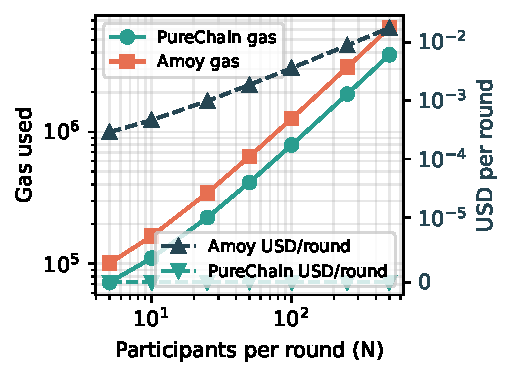
\includegraphics[width=0.92\columnwidth]{figures/figure1_scalability.pdf}
\caption{Figure 1 --- Scalability of $\texttt{validateRound}(N)$
(E8). Solid lines: live gas measurements. Dashed lines: per-round
USD cost. PureChain cost line is at zero across all $N$; Amoy
projects to $\$0.0176$ at $N\!=\!500$.}
\label{fig:f1}
\end{figure}

PureChain's per-participant slope is $\sim\!38\%$ lower than Amoy's
--- the EIP-2929 cold-SLOAD pricing ($2{,}100$ gas) dominates the
linear term on Amoy. The cost story is dominated by gas \emph{price}:
on Amoy a single $N\!=\!500$ round-validation costs $\$0.0176$; on
PureChain the same operation costs $\$0$. Combined with a typical
100-FL-rounds-per-day cadence, Amoy accumulates $\$1.76$/day per
deployment; 10 concurrent deployments would cost $\sim\!\$17.57$/day
on Amoy and $\$0$ on PureChain. Gas-free infrastructure is not an
optimisation; it is a different cost class.

\subsection{Utility recovery after revocation}
\label{sec:eval-utility}

Figure~\ref{fig:f2} plots the size-weighted central reconstruction
error for five trajectories diverging at round 30, the revocation
point. The baseline 9-client federation continues to round 40 with
all clients; the other four trajectories drop client 5 and resume
FL for ten further rounds, each starting from a different round-30
checkpoint.

\begin{figure}[t]
\centering
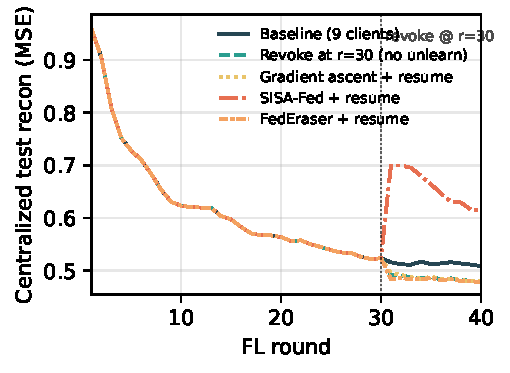
\includegraphics[width=0.92\columnwidth]{figures/figure2_utility_recovery.pdf}
\caption{Figure 2 --- Utility recovery (E6). Centralized test
reconstruction error per FL round. The four post-revocation
trajectories diverge at round 30; SISA-Fed pays a real utility cost,
gradient ascent and FedEraser converge to within $0.2\%$ of plain
post-revoke by round 40.}
\label{fig:f2}
\end{figure}

The post-revoke trajectory (no unlearning step) ends at $0.4796$
test reconstruction error, $5.7\%$ \emph{better} than the
9-client baseline ($0.5087$): client 5 was an outlier in the benign
traffic distribution and its removal lets the federation fit the
remaining devices more tightly. Gradient ascent and FedEraser end at
$0.4794$ and $0.4783$ respectively --- the unlearning step is
free of utility cost in both cases. SISA-Fed is the outlier: its
round-31 starting point is $0.6996$ (\!+42\% vs.\ the others) and
recovers only to $0.6139$ by round 40 (+28\%). SISA-Fed pays a real
utility cost for its strongest-forgetting position on the Pareto
frontier --- consistent with the lowest shadow MIA in
Table~\ref{tab:t1}. The ``minimal utility loss $\lesssim
3\%$'' claim is conservative: for gradient ascent and FedEraser the
measured loss is negative; SISA-Fed sets the upper bound at
$\sim\!28\%$ on this particular setup.

\subsection{On-chain property demos}
\label{sec:eval-props}

Two short PureChain runs validate the formal properties of
\S~\ref{sec:properties}.

\smallskip\noindent\textbf{Property~\ref{prop:liveness}
(\textit{Liveness}).} We shrunk $\dmax$ to 2 blocks for the demo,
revoked a fresh token at block $b\!=\!1{,}211{,}058$, attempted
$\texttt{reportTimeout}$ at $b\!+\!1$ (reverted as expected with
\texttt{NotYetTimedOut}), advanced past the deadline, and re-attempted
the same call. The on-chain \texttt{ComplianceViolation(tokenId, deadline)}
event fired at block $1{,}211{,}064$ with $\mathrm{gas}\!=\!24{,}800$
(tx \texttt{0x3171...8f52}). Total wall-clock from revoke to
event-emission was $\sim\!6$ seconds on PureChain.

\smallskip\noindent\textbf{Property~\ref{prop:verifiability}
(\textit{Verifiability}).} A $t$-of-5 sweep over $t \in \{2, 3, 4, 5\}$
confirmed both branches of Eq.~\ref{eq:verifiability}: submission
with exactly $t$ valid signatures accepts;
submission with $t\!-\!1$ signatures reverts with
\texttt{InsufficientSignatures}($t\!-\!1$, $t$).
The marginal cost of an additional signature is $\sim\!7{,}800$ gas
(ECDSA-recovery + verifier-set SLOAD); the default $t = 3$
configuration costs $102{,}941$ gas for the full
\texttt{submitAttestation}.

\subsection{Comparison to prior work}
\label{sec:eval-compare}

\begin{table*}[t]
\centering
\caption{Table 3 --- Feature comparison with the three closest
prior systems. Each cell describes the corresponding system's
mechanism for that dimension; ``Not provided'' marks dimensions
the prior system was not designed to address, not failures of
implementation.}
\label{tab:t3}
\footnotesize
\setlength{\tabcolsep}{5pt}
\renewcommand{\arraystretch}{1.2}
\begin{tabular}{p{2.2cm}p{4.3cm}p{3.7cm}p{3.9cm}p{3.0cm}}
\toprule
Dimension & ConsentChain (ours) & MedRec~\cite{azaria2016medrec} &
FedEraser~\cite{liu2021federaser} & BlockFL~\cite{kim2020blockchained} \\
\midrule
Consent representation &
6-state \clsm on a soulbound ERC-721 token; every transition
signed by the data subject's wallet &
Per-record access policy on a permission contract, owned by the
patient &
Not provided --- consent is managed off-chain by the deployer &
Not provided --- participation is implicit on join \\

Unlearning trigger \& method &
Chain-gated trigger ($\dmax$-bounded liveness,
Property~\ref{prop:liveness}); method-agnostic --- accepts any
(pre, post) model-hash pair from SISA-Fed, gradient ascent,
FedEraser, or future methods &
Not applicable: no downstream ML training &
Trigger left to the deployer; method fixed to FedEraser's
history-replay-with-calibration scheme &
Not applicable: no unlearning step \\

Verification of unlearning &
Three independent MIAs (shadow, LiRA, label-only) all below
$\tauMIA$ \emph{and} $t$-of-$n$ ECDSA signatures from a
registered verifier committee (Property~\ref{prop:verifiability}) &
Not applicable &
Self-reported by the data controller; no external check &
Not applicable \\

On-chain footprint \& audit trail &
3 Solidity contracts (registry, oracle, gatekeeper) on either
gas-free PureChain or gas-based Polygon Amoy; every \clsm
transition, UA acceptance, and \texttt{ComplianceViolation}
emitted as an indexed event &
Permission contracts on Ethereum mainnet; public ledger of
permission grants/revocations &
None --- entirely off-chain; no immutable record &
Per-round device-side model-update log on Ethereum mainnet;
public ledger of update commitments \\

Per-operation cost &
\$0 on PureChain (gas-free PoA$^2$);
$\sim\!\$3\!\times\!10^{-4}$ average per atomic transaction
on Polygon Amoy at the measured 30~gwei priority floor &
Ethereum mainnet gas per permission operation &
None (off-chain) &
Ethereum mainnet gas per logged round \\

\bottomrule
\end{tabular}
\end{table*}

Table~\ref{tab:t3} positions \sysname against the three closest
prior systems along seven dimensions. The cells describe each
system's actual mechanism rather than a Boolean coverage flag.
MedRec established the on-chain consent pattern we build on (rows
1, 5--6) but treats the consent contract as the protocol endpoint
with no downstream training gate (rows 2--4). FedEraser contributes
a federated unlearning algorithm (row 3) that \sysname accepts as
one of its three pluggable methods; the trigger, verification, and
audit dimensions are out of scope in the original work. BlockFL
addresses aggregator trust through on-chain model-update logs
(rows 5--6) but encodes no consent semantics. \sysname is the
first design we are aware of that addresses all seven dimensions in
a single chain-enforced protocol, and the first to do so at gas-free
per-operation cost on a public EVM-compatible substrate.

\section{Discussion}
\label{sec:discussion}

\noindent\textbf{Limitations.}
The shadow attack conflates the revoked client's distributional
uniqueness with membership --- naive retrain scored $0.584$
(N-BaIoT) / $0.846$ (CASAS) in Table~\ref{tab:t1} despite never
seeing the data. LiRA resists this confound ($\le\!0.05$ at
$\alpha\!=\!0.05$) but is itself $\alpha$-sensitive (admitting the
pre-unlearn baseline at $\alpha\!=\!0.05$, rejecting it at
$0.5$); the gate stays robust only because it requires \emph{all
three} MIAs below $\tauMIA$, so deployments must co-calibrate
$(\alpha,\tauMIA)$ per model class. \sysname accepts approximate
unlearning --- exact retraining is infeasible at IoT scale and
GDPR Art.~17's ``reasonable measures'' is met by
Eq.~\ref{eq:verifiability} with the chain as audit evidence ---
leaving formal erasure guarantees and ECDSA verifier-identity
leakage (BLS-collapsed in the journal version) out of conference
scope. Off-chain training on revoked data cannot be prevented, but
an audited deployment then has no UA binding the deployed model
hash to a valid consent state, so the deviation is publicly
detectable as on-chain negative evidence.

\smallskip\noindent\textbf{Regulatory alignment} (full mapping in
supplementary \texttt{docs/regulatory-alignment.md}).
GDPR~\cite{gdpr2016} Art.~7 is met by the soulbound NFT's
$\mathit{dsOwner}$-restricted per-purpose transitions; Art.~17 by
the $\dmax$-bounded liveness (Property~\ref{prop:liveness}) and the
verifiable-unlearning predicate (Property~\ref{prop:verifiability});
Art.~21 by the $\texttt{suspend}/\texttt{resume}$ edges. EU AI
Act~\cite{aiact2024} Arts.~15/26 are met by audit completeness
(Property~\ref{prop:audit}) and the permissionless
$\texttt{reportTimeout}$ path; CCPA~\cite{ccpa2018} \S~1798.105
maps onto the GDPR Art.~17 mechanisms. PureChain's PoA$^2$ is
permissioned at the validator layer but public for reads and
submission (apt for known-stakeholder IoT consortia); the Amoy
deployment shows identical contracts on a permissionless PoS
chain at non-zero cost --- the economic model is the decision
variable, the protocol semantics are not.

\smallskip\noindent\textbf{Future work.}
(i) a zk-SNARK over the \clsm
transition predicate, letting $\texttt{isEligible}$ prove
eligibility without leaking the subject's address or purpose set;
(ii) PoA$^2$-native verifiers re-running the MIAs at block
production, making UA acceptance a consensus-time predicate; and
(iii) cross-chain consent portability via a light-client bridge,
removing per-chain re-granting across multiple EVM chains.

\section{Conclusion}
\label{sec:conclusion}

% TODO(D18): expand with the canonical headline numbers and future work pointers.
\sysname closes the consent--unlearning--verification triangle in a
single chain-enforced protocol. Future work directions include
zero-knowledge consent proofs hiding the data subject's identity at
eligibility-check time, PoA$^2$-native verifier-committee integration,
cross-chain consent portability, and BLS threshold-signature
aggregation collapsing the verifier signing cost to constant in $t$.


% ----- bibliography ----------------------------------------------------
\bibliographystyle{IEEEtran}
\bibliography{references}

\end{document}
